\documentclass[10pt,conference,compsocconf]{IEEEtran}
\usepackage{graphicx}
\graphicspath{ {images/} }
\usepackage{combelow}
\usepackage{breqn}
\usepackage{multirow,tabularx}
\usepackage{booktabs}

\begin{document}

\title{A simple ensemble to leverage convolutional and recurrent neural networks}

\author{
  Drago\cb{s}-Alexandru ~Nica: 1791579\\
  Department of Computer Science, University of Warwick, UK
}

\maketitle

\section{Introduction}
\label{sec:introduction}

Mining social media data to determine people's sentiments is popular in the business sector. The technique can provide decisive insights for improving customer experience, marketing strategies, campaign success and so on. 

In this paper, the performance of two deep neural network architectures popularly used in sentiment analysis and their simple stacking ensemble model is assessed. Namely, the performance of a Convolutional Neural Network (CNN) and a Long Short Term Memory (LSTM) network are compared against a set of baseline models. The features are represented by TF-IDF weights and word embeddings both pre-trained and trained from scratch.

The dataset used for this work is the one for task 4-A of the 2017 Semeval competition.

\section{Text Preprocessing}
\label{sec:preprocessing}

The employed preprocessing techniques includes three main steps. Firstly, each tweet is tokenized. In the second part (pattern matching), elements which don't add any useful information are removed/replaced. In the third part, a spelling correction technique is used. 

\subsection{Tokenization} \label{subsec:tokenization}

Tokenizing a Twitter corpus can be a complex task due to the non-conventional way people use text on social media. Because of this, a specially designed module called "Twokenize" \cite{twokenize} was used for this task. Twokenize helps by identifying characters that appear exclusively on social media, such as emoticons ("=))", ":-(", ":o", etc.), abbreviations ("ikr", "smh", "lol", etc.) and missing characters ("you re" -$>$ "you're"). Furthermore, the Twokenize module automatically normalizes the raw Tweets data to unescape it from the HTML entities.

\subsection{Pattern matching} \label{subsec:pattern_matching}

To reduce the number of rare words while not removing useful information, a technique was implemented where words containing numbers are substituted by a "$<$number$>$" tag, URLs are substituted by a "$<$url$>$" tag, user mentions are replaced by the tag "$<$user$>$". For example, "watch @MichaelMoore in Trumpland 2016. I caught it on https://SHO2.com." will be transformed into "watch <user> in Trumpland $<$number$>$. I caught it on $<$url$>$.". 

In addition, hashtags are handled in a special way. A hashtag character ("\#") only followed by a string of digits (e.g. "\#104") is substituted with the "$<$number$>$" tag, since it provides no discriminant information. However, if that is not the case, next we check if the hashtag exists in a vocabulary of the word embeddings used in this work. If that is true, it probably means that the hashtag is frequent enough to add value in the training process. Nevertheless, very frequently people don't follow widely used hashtags and make up their own. To handle this case, hashtags which don't exist in the vocabulary are split in normal English words. 

Emoticons are also a strong indicator of the sentiment expressed in a tweet. Therefore, smile emoticons (i.e. in this work we consider smile emoticons to be ":)", ":-)", "\textasciicircum\_\textasciicircum") are grouped under one tag and replaced by "$<$smile$>$". In the same manner, sad face emoticons (":(", ":-(", ":((", ":-((") are subtituted by the "$<$sadface$>$" tag. Also, heart emoticons ("$<$3" and ":3") are subtituted by the "$<$heart$>$" tag and the laughing faces (":))", ":-))", ";))", ";-))") are subtituted by the "$<$lolface$>$". Because the the neutral face emoticon ("-\_-") does not exist in our vocabulary extracted from the GloVe Twitter 27B word embeddings, it is subtituted by the "$<$neutralface$>$" tag. 

\subsection{Text normalization} \label{subsec:text_norm}

To enhance the probability that the tokens from the tweets corpus can be mapped to a correct word in the our vocabulary, a spelling correction technique was trialled. 

The solution for spelling correction is based on the algorithm by Peter Norvig \cite{spelling_corrector}. The algorithm compares word derivations within 1 or 2 edit distances against the correct words from a language model. The language model is extracted from a large corpus for inferring the corrected word. For this work, the vocabulary contains only words which exist in the embeddings used for training. This is because the input tweets of the neural networks only contains words that are present in those embeddings. Therefore, skipping other words in the corpus' vocabulary minimizes the computational expense of building the language model and inferring the corrected words.

\section{Word Embeddings}
\label{sec:embeddings}

The Twitter version of the GloVe word vectors are used in the current version of this work \cite{glove_twitter}. The 25-dimensional pre-trained vector is used in the spelling correction step. For the LSTM and CNN models, only the 50, 100 and 200-dimensional GloVe representations are used due to their richness. 

In addition, the Google News word2vec embeddings were also used in training the models. These have 300 dimensions, hence they bring in more potentially useful information into the training process. Nonetheless, these word embeddings didn't improve the models' performance. Most likely, this is because the Google word2vec embeddings are extracted from a different distribution than the GloVe Twitter ones (news compared to tweets).

Training new embeddings from scratch was also tried. This method yielded the worst models performance compared to the above two. The results from training the models with new embeddings is not considered useful information, hence they were not included in this report.

\section{Baseline models}
\label{sec:baselines}

Three machine learning algorithms were first trained to build a baseline for comparison with the CNN and the LSTM network models. These baseline algorithms are: logistic regression (LGR), support vector machines (SVM) and a fully connected deep neural network (FCNN). 

The baseline models were trained on two types of features: TF-IDF and averaged word embeddings.

\subsection{Baselines + TF-IDF} \label{baselines_tfidf} 

First, TF-IDF features were extracted from the training corpus. The TF-IDF weight is computed for each token in the corpus using the following formula:

\begin {dmath} \label{eq:convolution}
w_{t,d} = \Big( 1 + log (tf_{t,d}) \Big) \times log_{10}\Big(\frac{N}{df_t} \Big)
\end{dmath}

where $tf_{t,d}$ is the frequency of the token $t$ in tweet $d$, $N$ is the number of tweets in the corpus and $df_t$ is the number of tweets in the corpus that contain the token $t$.

In this work, the terms which appear in less than $40\%$ of the tweets are removed, since they don't provide much discriminatory information. The resulting TF-IDF features are represented by a sparse matrix. This is because a tweet is usually a short sentence, but the corpus actually contains a high variety of words (378045 unique tokens).

\subsection{Baselines + averaged word embeddings} \label{baselines_we} 

Three sources of word embeddings were used throughout this work, as explained in section \ref{sec:embeddings}. For the baseline models, the embeddings for the words in each tweet were averaged. Therefore, each tweet being represented by a vector of the same dimension as the original embeddings it was extracted from.

\section{Convolutional Neural Network}
\label{sec:CNN}

CNNs were originally developed as classifiers for imagery data, such object detection, facial recognition, etc. However, they have also recently become popular in the Natural Language Processing (NLP) community, specifically in sentence classification problems. Their merit is their ability to extract the most important features (n-grams) in the embedding space. Figure \ref{fig:cnn_arch} illustrates the CNN architecture used in this work. The design choices are explained in the subsections \ref{subsec:input_layer_cnn}, \ref{subsec:conv_layer_cnn} and \ref{subsec:training_cnn}.

\begin{figure*}[h]
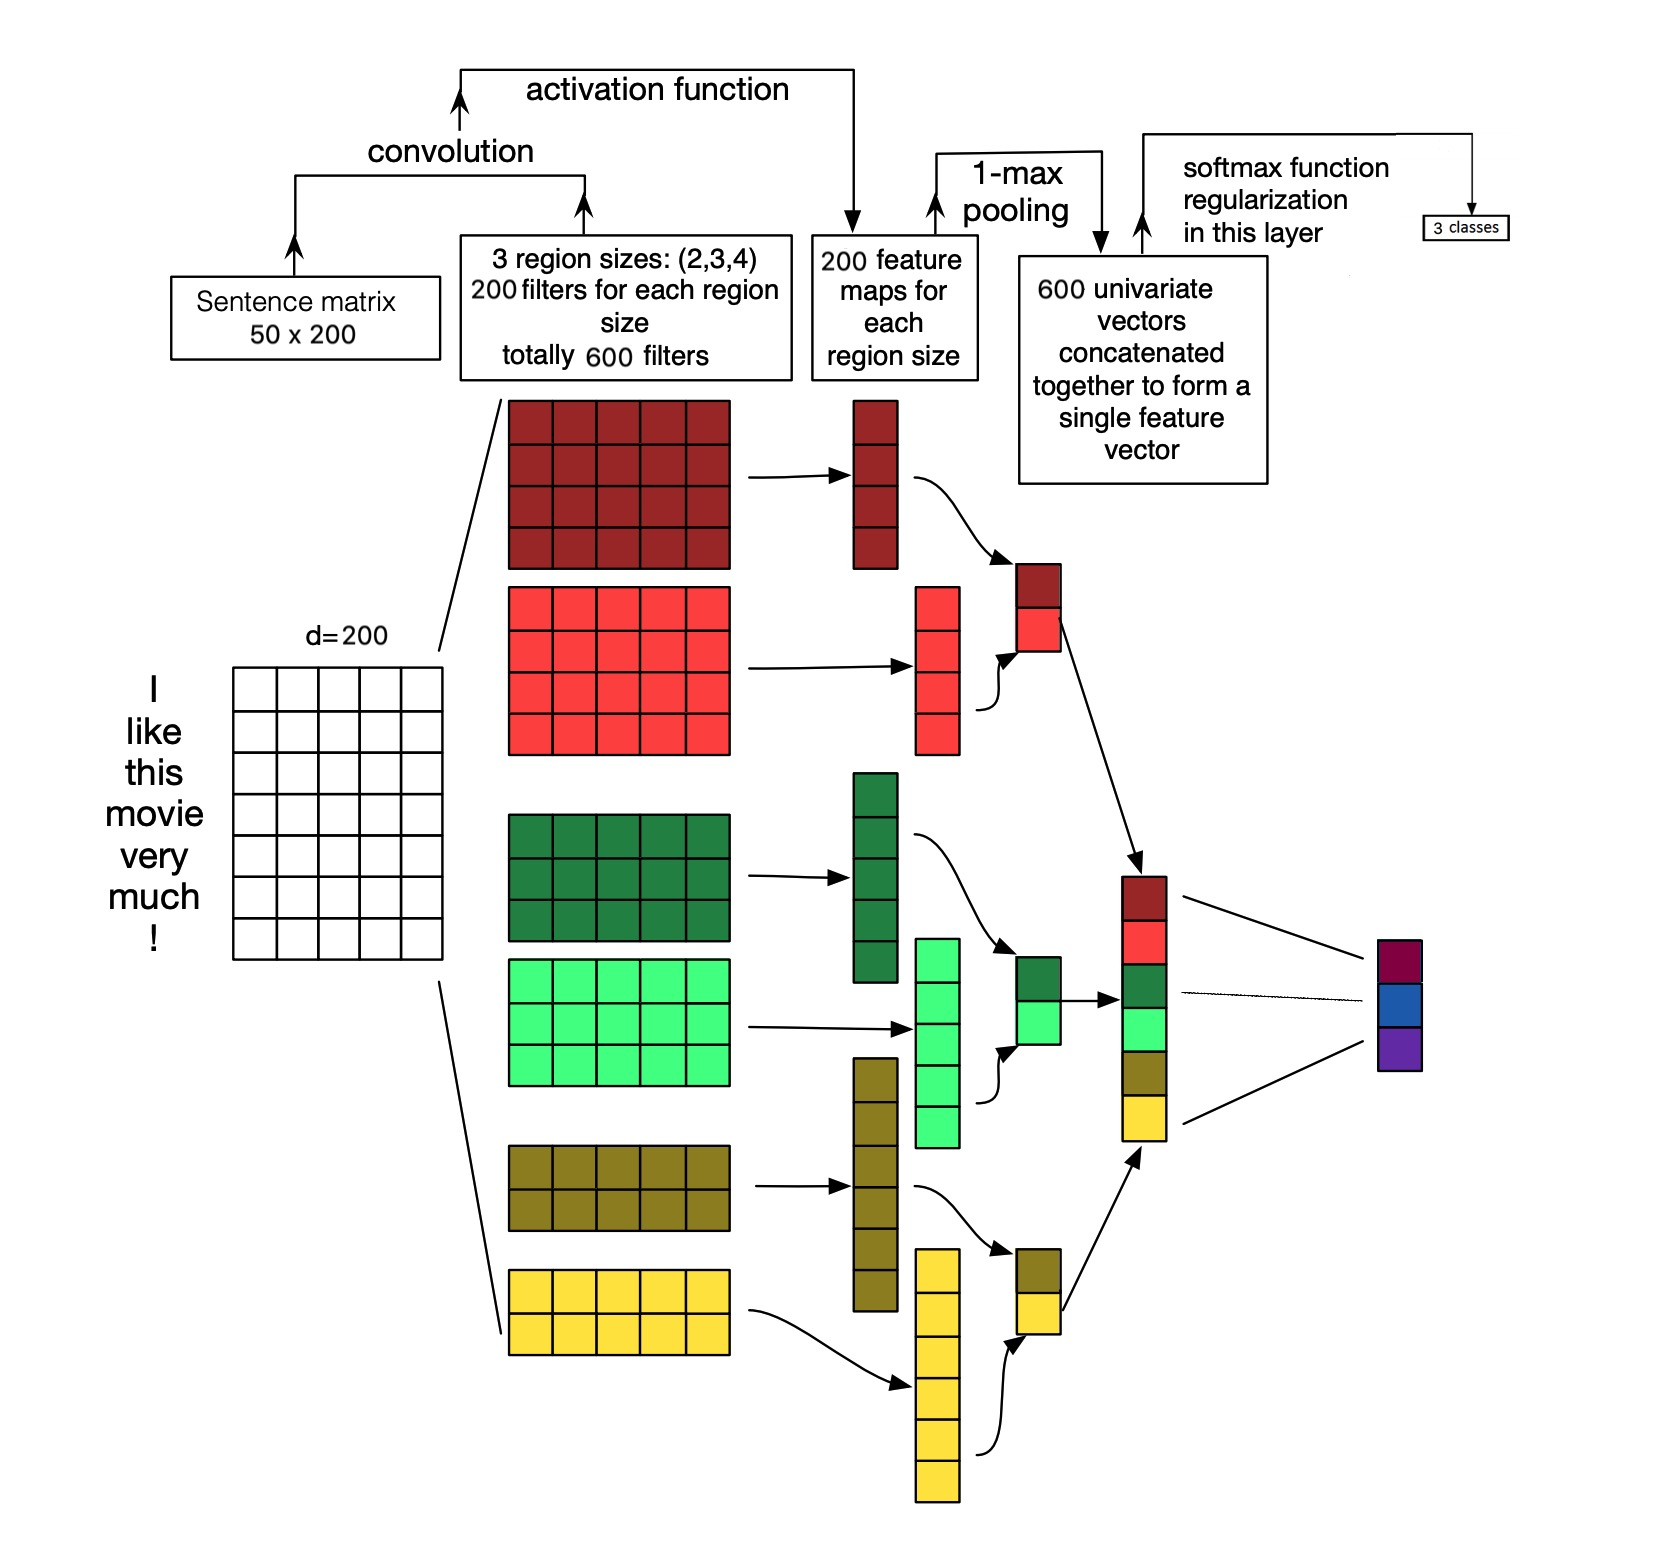
\includegraphics[width = 12cm, height = 10cm]{cnn_arch}
\centering
\caption{Architecture prototype of the CNN model. Final model also includes a fully connected layer before the softmax function. Original image is from Zhang and Wallace, 2015 \cite{cnn_sent_classification}}
\label{fig:cnn_arch}
\end{figure*}

\subsection{Input layer} \label{subsec:input_layer_cnn}

The convolutions require a invariable input dimensionality. Therefore, each tweet is limited to 50 words. Sentences with more than 50 words are clipped off and sentences with less than 50 words are padded with the $<$PAD$>$ token. 
Furthermore, each word is represented by a 50/100/200/300-dimensional pre-trained vector as explained in section \ref{sec:embeddings}. The word embeddings are also trained by the neural network during the main model's training process.

\subsection{Convolutional layer} \label{subsec:conv_layer_cnn}

A convolution is a sliding window (filter) which is shifted over the input matrix. Due to the nature of the data, the convolution is only performed on 1 dimension (over 1 sentence at a time). The convolution layer's operation is defined mathematically as:

\begin {dmath} \label{eq:convolution}
c_i =  h \Big( \sum_{j,k} w_{j,k} (X_{[i:i+h-1]})_{j,k} + b \Big)
\end{dmath}

where $h()$ is an activation function (rectified linear unit - ReLU chosen for this work), $X \in \rm I\!R ^{50\times d}$ is the matrix of word vectors of dimension $d$ covered by the filter of size $h$, $w_{j,k}$ is the weight in the filtering matrix $w \in \rm I\!R ^{h \times d}$ at position $(j,k)$ and $b$ is a bias term.

The model consists of 3 convolutional layers, each having a different filter size. Depending on the size of the filter, the convolution captures information from a bigram (filter size=2), trigram (filter size=3) or fourgram (filter size=4) per operation. Additionally, each layer makes use of 200 filtering matrices to learn a wide variety of features.

The convolutional layers use the same padding, meaning that the shape of the produced convolutions is constant throughout filtering. 

Each convolution layer is max-pooled to extract only the most important produced output from every convolution. Hence, each convolution layers output 3 200-dimensional vector, which are then concatenated into a 600 dimensional vector and fed into a fully connected layer with 30 nodes.

\subsection{Training and regularization} \label{subsec:training_cnn}

To reduce overfitting, a dropout layer is added between the fully connected layer and the softmax function. This layer drops connection in the fully connected layer with a probability of $50\%$.

The model is trained using stochastic optimization to minimize the cross-entropy loss. For this, the Adam optimizer was chosen, which is known to work generally well. The training accuracy, development accuracy, training loss and development loss were logged after every epoch. The best performing model was considered the one with the highest development accuracy. The algorithm would stop training after 5 epochs with no improvement in the dev accuracy.

\section{Long Short-Term Memory Network} 
\label{sec:LSTM}

The LSTM network is a type of recurrent neural network, which are a type neural network specifically designed to fit sequential data. Recurrent neural networks (RNNs) contain inter-node connections which form a directed graph. This means that the internal state of any network unit acts as memory. Since data is fed into the neural network sequentially, this memory function represents added value when the next bit of the sequence is fed into the network. A time $t$, the internal state $i_t$ of a unit is defined as:

\begin {dmath} \label{eq:convolution}
m_t = h (   W_m \cdot x_t + U_m \cdot m_{t-1} + b_m  )
\end{dmath}

where $W_m \in \rm I\!R ^{n \times d}$ represents the recurrent connection weight matrix at the previous and current hidden layers and $U_m \in \rm I\!R ^{n \times n}$ represents the weight matrix connecting the inputs to the current hidden layer. $n$ is the number of recurrent units in the network layer (200 in this work). $x_t$ is the word vector for the current token, $m_{t-1}$ is the previous state of the unit and $b_m \in \rm I\!R ^ n$ is a bias term. As with the convolutional operation, $h()$ is the activation function.

Nonetheless, RNNs have a reliability issue. Because they often have to send error signals over a large number of units during backpropagation, they often exhibit exploding or vanishing gradients. The advantange of LSTMs over other types of RNNs is that it alleviates the vanishing gradients by having a more complex internal function. Even though they are more complex than other RNNs, they can propagate the error signals in a more elegant manner.  The exploding gradients issue is usually resolved through clipping. The internal state of an LSTM unit is computed as follows:

\begin {dmath} \label{eq:lstm1}
f_t = \sigma ( W_f \cdot x_t + U_f \cdot m_{t-1} + b_f  )
\end{dmath}
\begin {dmath} \label{eq:lstm2}
i_t = \sigma ( W_i \cdot x_t + U_i \cdot m_{t-1} + b_i )
\end{dmath}
\begin {dmath} \label{eq:lstm3}
o_t = \sigma ( W_o \cdot x_t + U_o \cdot m_{t-1} + b_o )
\end{dmath}
\begin {dmath} \label{eq:lstm4}
C_t = \sigma \Big(C_{t-1} * f_t  + i_t * tanh(W_c \cdot x_t + U_c \cdot m_{t-1} + b_c)\Big)
\end{dmath}
\begin {dmath} \label{eq:lstm5}
m_t = tanh(C_t) * o_t
\end{dmath}

where $*$ is element-wise multiplication, $f_t$, $i_t$, $o_t$ are called the forget, input and output gates, respectively. These are the functions that control how much information is propragated to other units. $C_t$ is an explicit memory function of the unit. 

\subsection{Input layer} \label{subsec:input_layer_lstm}

The input layer for the LSTM network was prepared similarly to the one for the CNN (see subsection \ref{subsec:input_layer_cnn}). The input layer is a $32 \times 50 \times 200$ matrix, where 32 is the batch size, 50 is the sentence length and 200 is word embedding dimension the network performed best with. 

Just as with the CNN, the embeddings are also trainable by the network.

\subsection{LSTM layers} \label{subsec:lstm_layers}

\begin{figure*}[h]
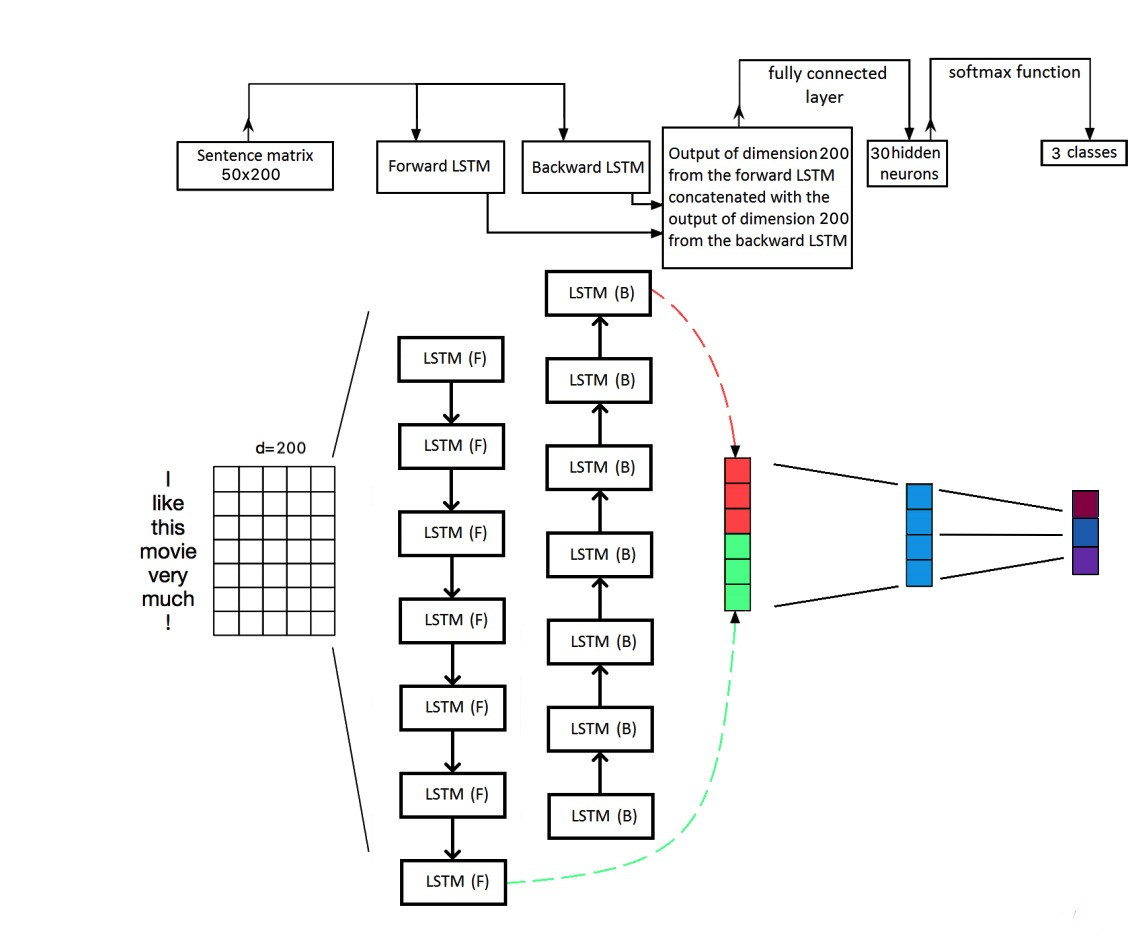
\includegraphics[width = 12cm, height = 10cm]{lstm_arch}
\centering
\caption{Architecture of the LSTM model. Final model also includes a fully connected layer before the softmax function. Original image is from Mathieu Cliche, 2017 \cite{BB_twtr_at_semeval}}
\label{fig:lstm_arch}
\end{figure*}

The mechanism described in section \ref{sec:LSTM} above only memorizes pre token information. This issue can be solved with bidirectional LSTM units (see figure \ref{fig:lstm_arch}). Bidirectional LSTM units are basically two stacked LSTM units, one reading a sequential input in a forward manner and another in a backward manner. 

The architecture of the LSTM network in this work contains two layers of 200 bidirectional LSTM units each. To alleviate the overfitting problem, a dropout layer is added on non-recurrent connection with a dropout probability of $50\%$. 

The output of the two layers of LSTM units is a concatenated vector with a length of 400 (200 from the forward LSTMs and 200 from the backward LSTMs). This is fed into a small fully connected layer of 30 nodes with a dropout probability of $50\%$. 

The final output is determined by a softmax function. 

\section{Stacking CNN + LSTM ensemble} \label{sec:ensemble}

A simple stacking ensemble model was trained to combine the predictions from two of the best CNN and LSTM models obtained. Since the performance of the CNN and the LSTM networks was just as good, a weighted average ensemble was not considered. Therefore, in the ensemble model both the CNN and the LSTM networks contribute equally. The intuition behind this model is that the two previously trained networks have learnt different features. Combining their forces into a third, meta-learner model means that when one fails to deliver a good prediction, the other will try to help.

The meta-learner model is made up of 3 fully connected layers. Two of the layers have 128 and 64 nodes respectively and the third layer is just a softmax function. Dropout reguralization is used after each layer to avoid overfitting. For the same reason, the training data for this model was not also used in training the CNN and LSTM models. 

The network input is a 6 dimensional vector containing the probabilistic predictions from the CNN and the LSTM networks (3 from each). 

\section{Results} 
\label{sec:results}

\subsection{Baselines} \label{subsec:baseline_results}

Table \ref{table:baseline_results} showcases the performance of these models.

\begin{table} \centering
\begin{tabular}[c]{ l c c c c}
	\toprule
	\multirow{2}{*}{\textbf{Model}} & \multicolumn{4}{c}{\textbf{Average}} \\
	 & \textbf{Train acc.} & \textbf{Dev acc.} & \textbf{Test acc.} &  \textbf{F1 score} \\
    \midrule
    LGR + TF-IDF & 0.912 & 0.657 & 0.643 & 0.490 \\
    \textbf{SVM + TF-IDF} & \textbf{0.962} & 0.650  & \textbf{0.649} & \textbf{0.560} \\
    FCNN + TF-IDF & 0.749 & \textbf{0.660} & 0.627 & 0.526 \\
    \midrule
    LGR + Av. WE & 0.595 & 0.606 & 0.609 & 0.472 \\
    SVM + Av. WE & 0.596 & 0.610  & 0.608 & 0.435 \\
    FCNN + Av. WE & 0.744 & 0.659 & 0.611 & 0.506 \\
   
    \bottomrule
\end{tabular}
\caption{Comparison table for the baseline models}
\label{table:baseline_results}
\end{table}

The logistic regression model with TF-IDF features massively overfit the training data. The same happened with the SVM + TF-IDF model. However, the SVM + TF-IDF model generated the best results on the test data from the chosen baselines, outperforming even the fully connected network with both TF-IDF and word embeddings features. 

It's interesting to note that the fully connected neural network still performed best amongst the models trained on averaged word embeddings. This is because of deep neural network's better ability to fit higher dimensional data than traditional machine learning models. The 200-dimensional GloVe embeddings proved to yield the best results for the baseline models.

\subsection{CNN, LSTM and ensemble models} \label{subsec:cnn_lstm_results}

\begin{table} \centering
\begin{tabular}[c]{ l c c c c}
	\toprule
	\multirow{2}{*}{\textbf{Model}} & \multicolumn{4}{c}{\textbf{Average}} \\
	 & \textbf{Train acc.} & \textbf{Dev acc.} & \textbf{Test acc.} &  \textbf{F1 score} \\
	\midrule
    CNN+Twtr GloVe & 0.770 & 0.683 & 0.670 & 0.592 \\
    CNN+GN word2vec & 0.712 & 0.670 & 0.642 & 0.500 \\
    \midrule
    LSTM+Twtr GloVe & 0.756 & 0.681 & 0.675 & 0.580 \\
    LSTM+GN word2vec & \textbf{0.794} & 0.680 & 0.668 & 0.554 \\
    \midrule
    \textbf{Ensemble+Twtr GloVe} & 0.775 & \textbf{0.690} & \textbf{0.687} & \textbf{0.596} \\
    Ensemble+GN word2vec & 0.770 & 0.682 & 0.672 & 0.550 \\
    \bottomrule
\end{tabular}
\caption{Comparison table for the CNN,  LSTM and ensemble networks}
\label{table:nn_results}
\end{table}

For the Twitter GloVe embeddings, the 200-dimension version help leverage the power of the deep neural networks best due to their richness. The Google News word2vec embeddings only exist in the 300-dimension format.

At the first sight, the LSTM network performed slightly better than the CNN. However, the lower F1 score indicates that this model has more bias than the CNN.

Combining the LSTM network and the CNN into a stacking ensemble model however, generated the best results.

\section{Discussion and summary} 
\label{sec:summary}

This work evaluated the performance of CNN, LSTM and simple stacking ensemble models in a multiclass sentiment classification problem. The deep learning literature trends have been confirmed by this work. LSTM networks generally manage to fit the training data better than a CNN. However, CNNs prove to be better at learning the importance of certain n-grams. Furthermore, naive ensemble models which only average probabilities enhance the performance of neural networks further and are very cheap to train. 

There are two possible ways that could be explored in the future in the quest to improve these results. Firstly, more CNN models could be trained to learn other n-grams (such as 5-grams, 6-grams, etc.) and their predictions be combined in a similar ensemble model as the one developed in this work. 

Another possible model to be developed is a joint CNN and LSTM ensemble model, where convolutions and max-pooling are followed by LSTM layers.

\bibliographystyle{IEEEtran}
\bibliography{semeval-tweets-report}
\end{document}
